\documentclass{article}

% if you need to pass options to natbib, use, e.g.:
%     \PassOptionsToPackage{numbers, compress}{natbib}
% before loading neurips_2019

% ready for submission
% \usepackage{neurips_2019}

% to compile a preprint version, e.g., for submission to arXiv, add add the
% [preprint] option:
%     \usepackage[preprint]{neurips_2019}

% to compile a camera-ready version, add the [final] option, e.g.:
     \usepackage[final]{neurips_2019}

% to avoid loading the natbib package, add option nonatbib:
%     \usepackage[nonatbib]{neurips_2019}

\usepackage[utf8]{inputenc} % allow utf-8 input
\usepackage[T2A]{fontenc}    % use 8-bit T1 fonts
\usepackage{hyperref}       % hyperlinks
\usepackage{url}            % simple URL typesetting
\usepackage{booktabs}       % professional-quality tables
\usepackage{amsfonts}       % blackboard math symbols
\usepackage{nicefrac}       % compact symbols for 1/2, etc.
\usepackage{microtype}      % microtypography
\usepackage[russian]{babel}

\usepackage{graphicx}
\graphicspath{{./images/}}

\title{Semi-supervised Learning with
Deep Generative Models\\
(воспроизведение результатов)}

% The \author macro works with any number of authors. There are two commands
% used to separate the names and addresses of multiple authors: \And and \AND.
%
% Using \And between authors leaves it to LaTeX to determine where to break the
% lines. Using \AND forces a line break at that point. So, if LaTeX puts 3 of 4
% authors names on the first line, and the last on the second line, try using
% \AND instead of \And before the third author name.

\author{%
  Даниил Гайдамашко \\
  БПМИ-161\\
  НИУ ВШЭ\\
  % examples of more authors
  \And
  Денис Сурин\\
  БПМИ-162\\
  НИУ ВШЭ\\
  % Coauthor \\
  % Affiliation \\
  % Address \\
  % \texttt{email} \\
  % \AND
  % Coauthor \\
  % Affiliation \\
  % Address \\
  % \texttt{email} \\
  % \And
  % Coauthor \\
  % Affiliation \\
  % Address \\
  % \texttt{email} \\
  % \And
  % Coauthor \\
  % Affiliation \\
  % Address \\
  % \texttt{email} \\
}

\begin{document}

\maketitle

\begin{abstract}
    В статье авторы пытались решить задачу частичного обучения с использованием генеративных моделей. 
    Своей целью они ставили при помощи небольшого размеченного датасета уметь получать результаты для намного большего количества неразмеченных данных. 
    К примеру, из датасета MNIST брали 50000(?) неразмеченных объектов и от 100 до 3000 размеченных, и на них запускали свой алгоритм (то есть объем неразмеченных мог на несколько порядков быть меньше размеченных). Непосредственно в статье авторы пробовали такой подход на задаче классификации(определение верной цифры по картинке).
\end{abstract}

\section{Описание задачи и используемых алгоритмов}

В качестве генеративных моделей использовался вариационный автоэнкодер с различными модификациями. 

Формально, поставлена следующая задача:
Наблюдаемые данные вида $(X, Y)$, где $x\in\mathbb{R}^D$, $y\in\{1, \dots, L\}$ сопоставляются некоторым латентным переменным $z$. 
В условиях частичного обучения метки известны только у некоторых объектов выборки.
Предположим, что величины $X$ генерируются из распределения $p_\theta(x|z)$. 

Чтобы найти по заданной выборке апостериорное распределение скрытых переменных $p_\theta(z|x)$, аппроксимируем его распределением $q_\phi(z|x)$.

Были предложены 3 модели: М1, М2 и М1 + М2. 
\subsection{M1}
В качестве априорного распределения латентных переменных берется $p(z) =  \mathcal{N}(z | 0, I)$.
Декодер строит распределение $p_\theta(x|z)=f(x;z, \theta)$, а энкодер аппроксимирует апостериорное при помощи $q_\phi(z|x)=\mathcal{N}(z|\mu_\phi(x), diag(\sigma_\phi(x)))$.
Функция потерь определим при помощи нижней оценки правдоподобия:
$$
\log p_\theta(x)
\geq
\mathbb{E}_{q_\phi(z|x)}\left[
    \log p_\theta(x|z)
    \right] - KL(q_\phi(z|x)||p_\theta(z))=-\mathcal{J}(x)
$$
где первая часть является reconstruction loss (считается при помощи reparametrization trick), а KL-loss выводится аналитически.

В М1 на вход энкодеру подавались как размеченные, так и неразмеченные данные. Энкодер представлял собой нейросеть с 2 скрытыми слоями (размерность 600) и слоем активации softplus. Далее мы получаем вектор средних mu и сигма - параметры нормального распределения, из которого семплируем вектор латентных переменных z. Z передается декодеру и по нему получаем конечный результат. После обучения автоэнкодера происходит обучение классификатора: сначала исходная картинка кодируется обученным энкодером и далее на ее результатах обучается классификатор (применяется только на размеченных данных).
\begin{figure}[htbp]
    \centering
    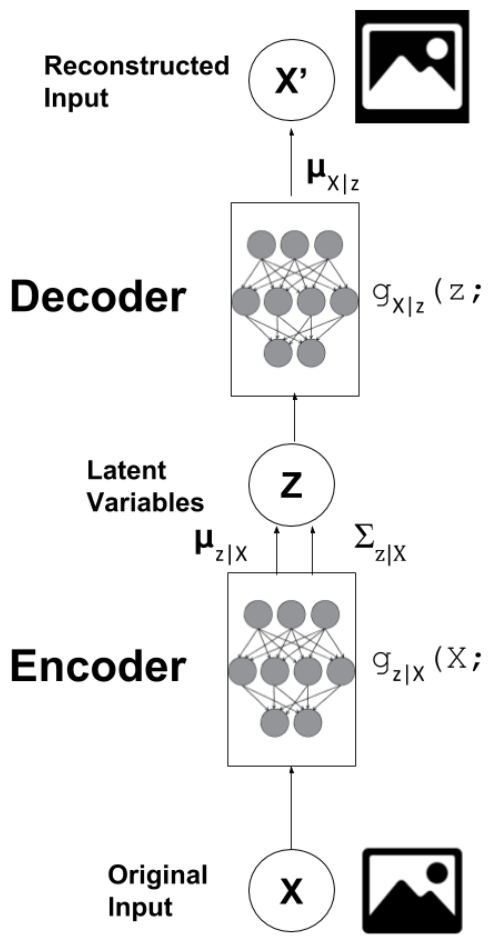
\includegraphics[scale=0.4]{m1}
    \caption{M1 архитектура}
\end{figure}

\subsection{M2}
Для построения распределения латентных переменных энкодером используются также и метки $y$. Вероятностная модель следующая:
$$
p(y)=Cat(y|\pi), \ 
p(z)=\mathcal{N}(z | 0, I) , \
p(x|y, z)=f_\theta(x, y, z, \theta)
$$
Если говорить менее формально, М2 в автоэнкодере идет разделение: размеченные данные обучаются на классификаторе, неразмеченные - в энкодере - и латентные переменные z получаются из распределения, зависящего и от x и от y. Итоговое предсказание получается при помощи обучившегося классификатора.
\begin{figure}[htbp]
    \centering
    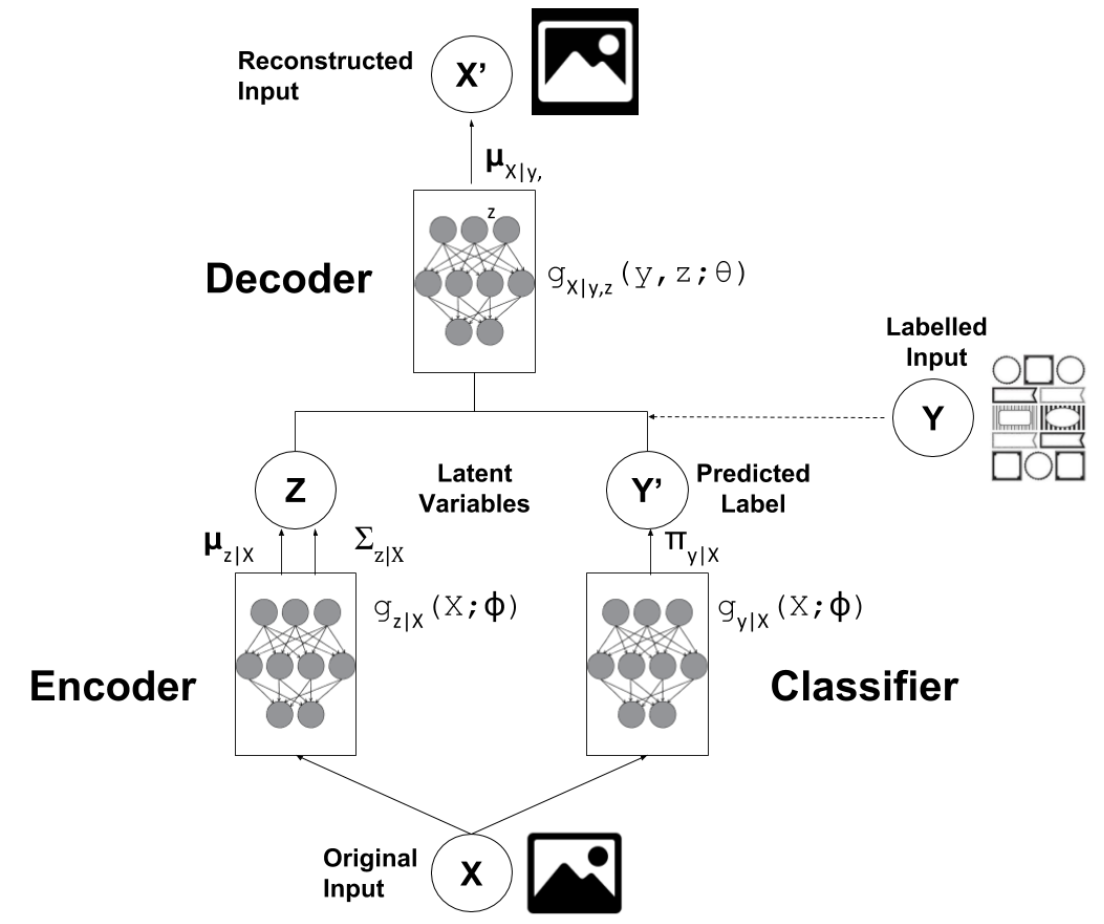
\includegraphics[scale=0.4]{m2}
    \caption{M2 архитектура}
\end{figure}
\subsection{M1 + M2}
Данная архитектура объединяет предыдущие подходы: на вход модели M2 подается новая латентная переменная $z_1$, полученная в результате обучения модели M1.
$$
p(x, y, z_1, z_2)=p(y)p(z_2)p_\theta(z_1|y, z_2)p_\theta(x|z_1).
$$
\begin{figure}[htbp]
    \centering
    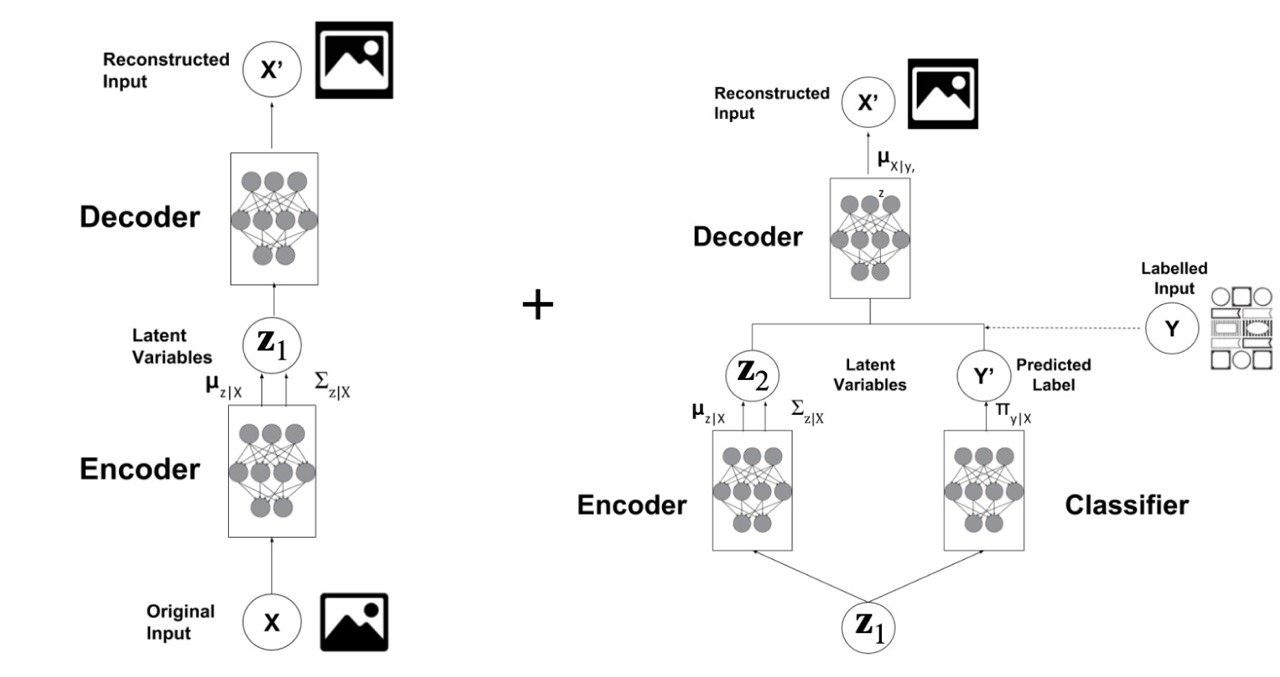
\includegraphics[scale=0.3]{m1+m2}
    \caption{M1+M2 архитектура}
\end{figure}
\section{Данные}
Авторы проводили эксперименты на датасетах MNIST, SVNH, NORB. 
Нашей текущей задачей было провести эксперименты только на датасете MNIST моделей М1, М2. 
Данные были нормализованы и разбиты на тестовую и обучающую выборки стандартными средствами Pytorch. 

\section{Подзадачи}
На текущей момент стояло 2 подазадачи: реализовать модели М1 и М2, протестировать их на датасете MNIST. Модели были реализованы, в качестве гиперпараметров были взяты значения, указанные авторами статьи. Веса обеих моделей так же были проинициилизированы как указано в статье. В качестве нормирующей костанты в Reconstruction loss было взято значение C = 0.5. В результатах приведены данные при N - число размеченных объектов - = 3000. Мы пробовали проводить тестирование при других значениях N, значительно отличающихся результатов получено не было.

\section{Результаты}
Полученные результаты пока что отличаются от авторских. Это можно объяснить тем, что в статье было довольно немного деталей реализации и если основная архитектура была бегло указано, как и некоторые гиперпараметры, то функция потерь была указана лишь аналитически, поэтому детали реализации могут значительно отличаться от авторских, что приводит к более худшим в сравнении с авторскими (у них лосс был порядка 11) результатам.
\begin{figure}[htbp]
    \centering
    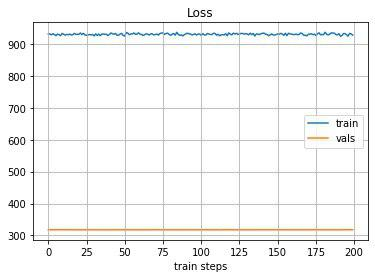
\includegraphics[scale=0.6]{data}
    \caption{M1 кривая обучения (accuracy$\approx 0.1$)}
\end{figure}
\begin{figure}[htbp]
    \centering
    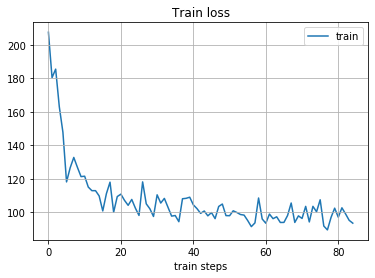
\includegraphics[scale=0.6]{train}
    \caption{M2 кривая обучения на обучающей выборке}
\end{figure}
\begin{figure}[htbp]
    \centering
    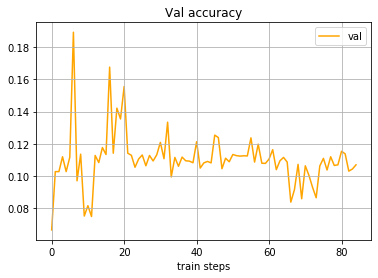
\includegraphics[scale=0.6]{val}
    \caption{M2 метрика accuracy на валидационной выборке}
\end{figure}
\newpage
\section{Дальнейшие планы}
Следующим заданием является реализация М1 + М2 модели и тестирование на 2 датасетах - MNIST и SVHN. Так же после получения обратной связи надеемся суметь улучшить существующие модели.  

\section{Ссылка на репозиторий}
\url{https://github.com/Haidaansko/SSL-VAE}
\end{document}